Today's lecture provides an introduction to nonlinear dynamics. 

\subsection{Key Concepts}
\subsubsection{Definitions}

\begin{definition}
    \textbf{Dynamical system} : A dynamical system is a deterministic mathematical formulation for evolving the state of a system forward in time.
\end{definition}

\begin{definition}
    \textbf{State of a system} : The state of a system is given by a variable $\bm{x}$, where $\bm{x}$ could be a vector (in this case $\bm{x} = \vec{x} = (x_1,x_2,...,x_n)^T$) or a continuous variable (in which case $x = f(\vec{r})$)
\end{definition}

At $t=0$ we have $x(0) = x_0$, the dynamical system then tells us how we get to $x(t)$, $\forall t > 0$. We consider two different representations of time, it can be: 
\begin{enumerate}
    \item \textbf{discrete}, in which case $t \in \mathbb{Z}_+$ and we call the system a \textit{discrete dynamical system},
    \item \textbf{continuous}, in which case $t \in \mathbb{R}_+$, in which case we call the system a \textit{continuous dynamical system}.
\end{enumerate}

When a system depends on time in a continuously differentiable manner we call the system a \textit{smooth dynamical system}. For now we will focus on \textit{continuous dynamical system}.\\

\noindent
\textbf{Continuous Dynamical Systems}: if $\vec{x}$ is a vector of, we can describe the dynamical system by a system of ODE, if $x(\vec{r})$ is continuous, we can describe the system by a system of PDE. PDE are much harder to deal with and we will mostly worry about ODEs in this course.  \\

\noindent
\textbf{General framework for a system of ODE}: 
\begin{definition}
    \textbf{N$^\textbf{th}$ order autonomous system:}\\
    Sometimes also referred to as \textit{N-dimensional autonomous system} or \textit{N-dimensional time-independent system}.

    \begin{align}
        \vec{F}(\vec{x}) = \vec{\dot{x}} =\frac{\partial \vec{x}}{\partial t} =
        \begin{cases}
            \frac{dx_1}{dt} = \dot{x}_1 = f_1(x_1,...,x_n) \\
            \frac{dx_2}{dt} = \dot{x}_2 = f_2(x_1,...,x_n) \\
            \vdots \\
            \frac{dx_n}{dt} = \dot{x}_n = f_n(x_1,...,x_n)
        \end{cases} 
        \tag{$\bigstar$}
    \end{align}
\end{definition}    
Any system of ODE can be ported into the form ($\bigstar$).\\

\begin{example}
    Let's take the non-linear driven-pendulum equation, how can we bring it into the form ($\bigstar$). Recall the equations are of the form: 
    \begin{center}
        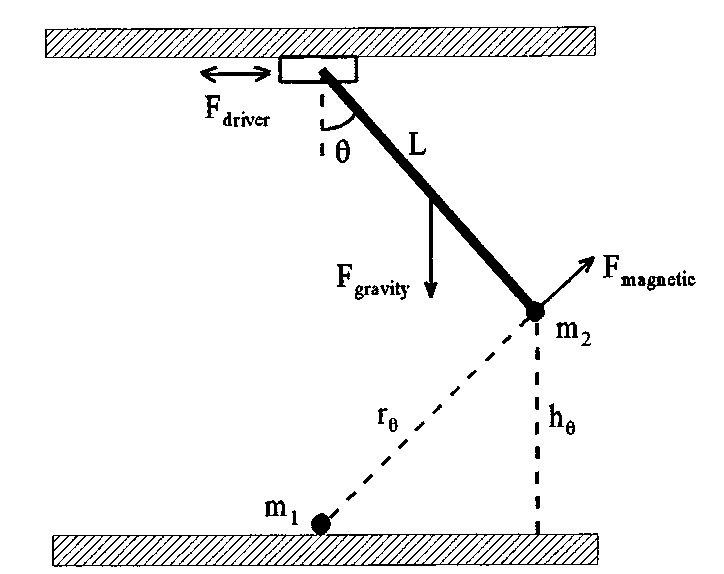
\includegraphics[width=0.3\textwidth]{figures/2_pendulum.png}
    \end{center}
    \[ \ddot{x} + \frac{g}{l} \sin(x) = \frac{F}{m} \cos(\Omega t) \]
    We define a 3-dimensional vector $\vec{x} = (x_1,x_2,x_3)^T$ such that:
    \[ 
      \dot{\vec{x}} = 
        \begin{cases}
            \dot{x}_1 = x_2\\
            \dot{x}_2 = -\frac{g}{l} \sin(x_1) + \frac{F}{m} \cos(\Omega x_3)\\
            \dot{x}_3 = 1
        \end{cases}.
    \]
    The way to think about this is that $x_1 = x$, $x_2 =\dot{x}$, $x_3 = t$ (since $\int 1 dt = t$).
\end{example}

\textit{Why would we want to get rid of time? There is actually a reason to do that.} Non autonomous systems have a dependance on time. When we solve a system of this type we get a vector of the form:

\[ \vec{x}(t) = \begin{bmatrix}
    x_1(t) \\
    x_2(t) \\
    \vdots \\
    x_n(t)
\end{bmatrix}, \]

which we call a \textit{trajectory} (or \textit{orbit}), this is a curve in \textit{phase-space}. The phase-space is completely filled with trajectories (i.e any point can be used as an initial condition point $\vec{x}_0$).

\begin{center}
    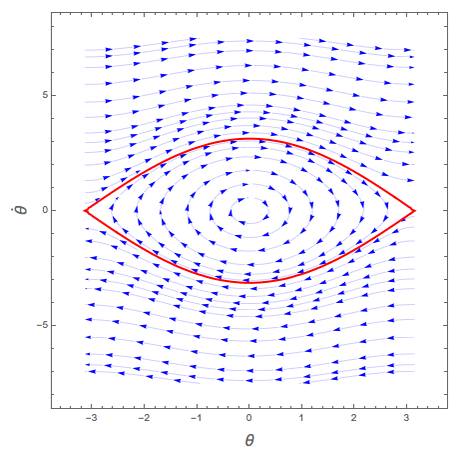
\includegraphics[width=0.4\textwidth]{figures/2_phase_space.png}
\end{center}

This is why we care about autonomous systems. Because time is present if the phase space (if required), we are guaranteed that the system is deterministic (with uniques solutions), there is no "crossing" in the phase space. \\

This enables us to express the solution as: 

\[ \phi(\vec{x}_0,t), \]

which we call \textit{flow} of the dynamical system. The flow has two key properties.

\begin{property}
    $\phi(\vec{x}_0,0) = \vec{x}_0$
\end{property}
\begin{property}
    $\phi(\phi(\vec{x}_0,t),s) = \phi(\vec{x}_0,t+s)$
\end{property}

\begin{example}
    The function $\phi(x_0,t) = x_0 e^t$ is the flow of the ODE $\dot{x} = x$.
\end{example}

\subsubsection{Existence and Uniqueness of a Solution}

Given a system of ODE:

\[ \frac{\partial \vec{x}}{\partial t} = \vec{F}(\vec{x}). \]

\textit{We ask ourselves under which conditions there exists a solution that satisfies $\vec{x}(0) = \vec{x}_0$ and it is unique.}

\begin{example}
    Consider the following system: 
    \begin{align*}
        \frac{dx}{dt} = 
        \begin{cases}
            1 & \textit{ if } x < 0 \\
            -1 & \textit{ if } x \geq 0 
        \end{cases}.
    \end{align*}
    No solution satisfies $x(0)=0$ because a solution of this kind would have to decrease ($x(0) = -1$) but $\forall x < 0$ it should increase ($x(x<0) = 1$).
\end{example}

\begin{example}
    Consider the leaky bucket equation: 
    \begin{align*}
        \dot{x} = - \sqrt{x}.
    \end{align*}
    That derives from Bernoulli $\frac{v^2}{2} + gx + \frac{p}{\rho} = \text{constant}$. The solution of the leaky bucket equation is:
\begin{align*}
    x(t) = 
    \begin{cases}
    \frac{1}{4} (t-c)^2 & \textit{ for } t < 0 \\
    0 & \textit{ for } t \geq 0 
    \end{cases}.
\end{align*}
\end{example}

\noindent
\textbf{Reminders}

\begin{definition}
    \textbf{Uniform convergence :} suppose we have some sequence of functions. $x_k(t)$, $k=0,1,2...$ is a sequence of $C^0$ functions which are defined in a time-interval $t \in [t_0,t_1]$, let's assume that given $\epsilon > 0$ there is $N>0$ s.t. $\forall p,q > N$, $\max_{t \in [t_0,t_1]} |x_p(t),x_q(t)| < \epsilon$. Then there is a $C^0$ function $x(t)$ for $t \in [t_0,t_1]$ such that: 
    \[
        \max_{[t_0,t_1]} |\vec{x}_k(t) - \vec{x}(t)| \rightarrow 0 \text{ as } k \rightarrow \infty
    \]
\end{definition}


\begin{definition}
    \textbf{Lipschitz Functions :} $\vec{F}$ is said to be \textit{Lipschitz} in $I$ if $\exists$ a constant $L$ s.t. $|\vec{F}(\vec{x})-\vec{F}(\vec{y})| \leq L |\vec{x}-\vec{y}|$ $forall x,y \in I$. \\

    $L$ is called the Lipschitz constant. Note : if $F$ is $C^1$ in $I$, with $I$ compact (closed and bounded), then $F$ is Lipschitz in $I$.
\end{definition}

This brings us to the main theorem of this lecture (which we are going to prove):

\begin{theorem}
    \textbf{Existence and uniqueness of the solution :} consider $\frac{d\vec{x}}{dt} = \vec{F}(\vec{x})$, with $\vec{x}(0)= \vec{x}_0$. \\

    If the following are true:
    \begin{enumerate}[label=(\roman*)]
        \item  $\vec{F}$ is defined on $I$, $I$ being the set of points s.t. $|\vec{x} - \vec{x}_0|< \rho$,
        \item there is a Lipschitz constant $L$ for $\vec{F}$ on $I$,
        \item $|\vec{F}(\vec{x})| \leq M$ on $I$ (has a maximum),
    \end{enumerate}
    then there is a unique solution $\vec{x}$ defined as a mapping $t \in [-a,a] \rightarrow I$. When $a \leq \min \left( \frac{\rho}{M}, \frac{1}{L} \right)$, s.t. $\vec{x}(0)= \vec{x}_0$.
\end{theorem}

\begin{proof}
    We will use the Picard iteration. Consider a sequence of functions $\vec{x}_0 (t), \vec{x}_1 (t), ...,\vec{x}_k (t)$ defined as :
    \begin{align*}
        \vec{x}_0(t)  = \vec{x}_0 \text{ , for $t \in [-a;a]$} \\
        \vec{x}_1(t)  = \vec{x}_0 + \int_0^t \vec{F}(\vec{x}_0(s)) ds = t + \vec{F}(\vec{x}_0)\\
        \vdots \\
        \vec{x}_{k+1}(t)  = \vec{x}_0 + \int_0^t \vec{F}(\vec{x}_k(s)) ds.
    \end{align*}

    We show that:
    \begin{enumerate}[label=(\alph*)]
        \item That the sequence is defined ($x_k \in I$) for $t \in [-a,a]$, $\forall K$. 
        \item It's uniformly convergent. 
        \item It converges to the solution of $\frac{\partial \vec{x}}{\partial t} = \frac{\vec{F}}{\vec{x}}, \vec{x}(0) = \vec{x}_0$.
        \item The solution is unique.
    \end{enumerate}

    \noindent (a) let's show the sequence can be defined: \\

    Since $|t| \leq a$, $|\vec{F}(\vec{x})| \leq M$, $|\vec{x}_1(t) - \vec{x}_0| = |t| \cdot |\vec{F}(\vec{x}_0)| \leq a M$. The claim is trivially true for $x_0(t)$ and $x_1(t)$, we will use induction to prove it for $k>1$. \\

    Assume that $x_k(t) \in I \Rightarrow |\vec{x}_k(t) - \vec{x}_0| \leq \rho$, for $t \in [-a,a]$, then $|\vec{x}_{k+1}(t) - \vec{x}_0| \leq \rho$ is what we need to show.

    \begin{align*}
        |\vec{x}_{k+1}(t) - \vec{x}_0| = |\int^t_0 \vec{F}(\vec{x}_k(s)) ds| \\
        \leq \int^t_0 |\vec{F}(\vec{x}_k(s))| ds \leq  \int^t_0 M ds \leq  M a
    \end{align*}
    now since we have $a < \frac{\rho}{M}$ $\Rightarrow$ $|x_{k+1} - x_0| < \rho$ so $x_{k+1} \in I$, $\forall t \in [-a,a]$, $\forall k > 0$. (The Picard iteration exists and has some value). \\

    \noindent (b) let's show uniform convergence: \\

    Let $R$ be the maximum of $|x_1(t)-x_0|$ for $t \in [-a,a]$, ($R \leq aM$), now let's study what happens between $x_2$ and $x_1$. $|\vec{x}_2 - \vec{x}_1| = |\int_0^T \left[ \vec{F}(\vec{x}_1) - \vec{F}(\vec{x}_0) \right]|$. \\ 

    Now recall that $F$ is Lipschitz:
    \begin{align*}
        |\vec{x}_2 - \vec{x}_1| = |\int_0^T \left[ \vec{F}(\vec{x}_1) - \vec{F}(\vec{x}_0) \right]|\\
        \leq \int_0^T L |\vec{x}_1(s) - \vec{x}_0(s)| ds \leq aLR,
    \end{align*}

    one can then prove by induction that $|\vec{x}_{k+1} - \vec{x}_k| \leq (aL)^k R$, since $a \leq \min \left( \frac{\rho}{M}, \frac{1}{L} \right) \Rightarrow aL < 1$, one can prove that given $\epsilon > 0$, we can choose $N$ such that for $R,S > 0$, $|\vec{x}_R(t) - \vec{x}_S(t)| < \epsilon$ $\Rightarrow$ $\vec{x}_k(t) \rightarrow x(t)$ (as $k \rightarrow \infty$). \\

    \noindent (c)  show that our system actually converges to the solution of the ODE system: \\

    Just look at the formulation for the Picard iteration: 

    \begin{align*}
        \vec{x}_{n+1}(t) = \vec{x}_0 + \int_0^t \vec{F}(\vec{x}_k(s))ds,
    \end{align*}

    take $k \rightarrow \infty$, we get:

    \begin{align*} 
        \vec{x}(t) = \vec{x}_0 + \int^t_0 \vec{F}(\vec{x}(s)) ds.
    \end{align*}

    The we just verify that this indeed is the flow in two steps: 

    \begin{enumerate}[label=(\roman*)]
        \item $\vec{x}(0) = \vec{x}_0 + \int^0_0 \vec{F}(\vec{x}(s)) ds =  \vec{x}_0$,
        \item $\frac{\partial \vec{x}}{\partial t} = \frac{\partial}{\partial t} \vec{x}_0 + \frac{\partial }{\partial t}\int^t_0 \vec{F}(\vec{x}(s)) ds =  \vec{F}(\vec{x}(t))$ by the fundamental theorem of calculus.
    \end{enumerate}

    which proves that indeed the Picard iteration provides a solution to the ODE system.

    \noindent (d)  NOT DONE IN 2021.

\end{proof}

Let's now got through a few examples of Picard iteration for the solutions of dynamical system.

\begin{example}
    $\frac{dx}{dt} = x$, with $x(0) = x_0$. \\ 
    
    Let's compute the first few Picard iterations:
    \begin{align*}
        x_0(t) = x_0\\
        x_1(t) = x_0 + \int_0^t F(x_0(s)) ds = x_0 + \int_0^t x_0 ds = x_0 + x_0 t  \\
        x_2(t) = x_0 + \int_0^t F(x_1(s)) ds = x_0 + x_0 t + x_0 t^2 \\
        \vdots \\
        x_k = x_0 \sum^k_{i=0} \frac{t!}{i!}
    \end{align*}
    which is just the Taylor expansion of $x_0 e^t$, $\lim_{k \rightarrow \infty} x_k = x_0 e^t$. 
\end{example}

\begin{example}
    $\dot{x} = - \sqrt{x}$. Note that as $-\sqrt{x} \rightarrow \infty$ as $x \rightarrow 0$, the $F$ is not Lipschitz. Therefore, we can't guaranteed that a solution exists.
\end{example}

During this semester, we will assume that the $\vec{F}$ we consider is sufficiently smooth so that a unique solution always exists. 

\subsubsection{Continuous Dependance on the Parameters}

We can ask ourselves \textit{"if I starts with an initial condition which is slightly different, will the solution be completely different"}, as one can imagine, this question is deeply related to the very notion of chaos and will be of great importance further in the course. 

\begin{theorem}
    Consider $\frac{\partial \vec{x}}{\partial t} = \vec{F}(\vec{x})$, with $\vec{F}$ is $C^1$, with solution $\vec{x}(t)$ s.t. $\vec{x}(0) = \vec{x}_0$, then, there exists a neighborhood $U$ of $\vec{x}_0$ and a constant $k$ such that if $\vec{y}(t)$ is another solution of the system s.t. $\vec{y}(0) = \vec{y}_0$ and $\vec{y}_0 \in U$, then:
    \begin{align*}
        |\vec{y}(t) - \vec{x}(t)| \leq k |\vec{y}_0 - \vec{x}_0|e^{kt}.
    \end{align*}    
\end{theorem}

We will not prove that theorem or the following claims in that course. 

\begin{lemma}
    If $\vec{\phi}(t,\vec{x}_0)$ is the flow of the system $\frac{\partial \vec{x}}{\partial t} = \vec{F}(\vec{x})$ and $\vec{F}$ is $C^1$, then $\vec{\phi}$ is a continuous function of $\vec{x}_0$.
\end{lemma}

\begin{example}
    The flow of $\dot{x} = x$ is $x=\phi(x,t)=x_0 e^t$ which is continuous w.r.t. $x_0$.
\end{example}

\noindent More generally:

\begin{lemma}
    If $\frac{\partial \vec{x}}{\partial t} = \vec{F}(\vec{x},a)$ depends on some (fixed) parameters $\vec{a}$ and $\vec{F}$ is $C^1$, then the flow depends continuously on $a$.
\end{lemma}